% This file was converted to LaTeX by Writer2LaTeX ver. 1.0.2
% see http://writer2latex.sourceforge.net for more info
\documentclass[twoside,letterpaper]{article}
\usepackage{amsmath}
\usepackage{amssymb,amsfonts,textcomp}
\usepackage{array}
\usepackage[english]{babel}
\usepackage[small,bf]{caption}
\usepackage{color}
\usepackage[T1]{fontenc}
\usepackage{hhline}
\usepackage{hyperref}
\usepackage[latin1]{inputenc}
\usepackage{multirow}
\usepackage{supertabular}
\hypersetup{pdftex, colorlinks=true, linkcolor=blue, citecolor=blue, filecolor=blue, urlcolor=blue, pdftitle=SYSTEMS AND SOFTWARE REQUIREMENTS SPECIFICATION (SSRS) TEMPLATE, pdfauthor=Clinton Jeffery, pdfsubject=, pdfkeywords=}
\usepackage[pdftex]{graphicx}
% Outline numbering
\setcounter{secnumdepth}{5}
\renewcommand\thesection{\arabic{section}}
\renewcommand\thesubsection{\arabic{section}.\arabic{subsection}}
\renewcommand\thesubsubsection{\arabic{section}.\arabic{subsection}.\arabic{subsubsection}}
\renewcommand\theparagraph{\arabic{section}.\arabic{subsection}.\arabic{subsubsection}.\arabic{paragraph}}
\renewcommand\thesubparagraph{\arabic{section}.\arabic{subsection}.\arabic{subsubsection}.\arabic{paragraph}.\arabic{subparagraph}}
\makeatletter
\newcommand\arraybslash{\let\\\@arraycr}
\makeatother
% Page layout (geometry)
\setlength\voffset{-1in}
\setlength\hoffset{-1in}
\setlength\topmargin{0.5in}
\setlength\oddsidemargin{1in}
\setlength\evensidemargin{1in}
\setlength\textheight{8.278in}
\setlength\textwidth{6.5in}
\setlength\footskip{0.561in}
\setlength\headheight{0.5in}
\setlength\headsep{0.461in}
% Footnote rule
\setlength{\skip\footins}{0.0469in}
\renewcommand\footnoterule{\vspace*{-0.0071in}\setlength\leftskip{0pt}\setlength\rightskip{0pt plus 1fil}\noindent\textcolor{black}{\rule{0.25\columnwidth}{0.0071in}}\vspace*{0.0398in}}
% Pages styles
\makeatletter
\newcommand\ps@Standard{
  \renewcommand\@oddhead{\rmfamily University of Idaho CS Department Instructional Use\hfill \hfill NOT FOR RELEASE}
  \renewcommand\@evenhead{\@oddhead}
  \renewcommand\@oddfoot{\foreignlanguage{english}{\textcolor{black}{SSRS Page }}\foreignlanguage{english}{\textcolor{black}{\thepage{}}}}
  \renewcommand\@evenfoot{\@oddfoot}
  \renewcommand\thepage{\arabic{page}}
}
\newcommand\ps@Convertviii{
  \renewcommand\@oddhead{}
  \renewcommand\@evenhead{\@oddhead}
  \renewcommand\@oddfoot{}
  \renewcommand\@evenfoot{\@oddfoot}
  \renewcommand\thepage{\arabic{page}}
}
\newcommand\ps@Convertvii{
  \renewcommand\@oddhead{}
  \renewcommand\@evenhead{\@oddhead}
  \renewcommand\@oddfoot{}
  \renewcommand\@evenfoot{\@oddfoot}
  \renewcommand\thepage{\arabic{page}}
}
\newcommand\ps@Convertvi{
  \renewcommand\@oddhead{}
  \renewcommand\@evenhead{\@oddhead}
  \renewcommand\@oddfoot{}
  \renewcommand\@evenfoot{\@oddfoot}
  \renewcommand\thepage{\arabic{page}}
}
\newcommand\ps@Convertv{
  \renewcommand\@oddhead{}
  \renewcommand\@evenhead{\@oddhead}
  \renewcommand\@oddfoot{}
  \renewcommand\@evenfoot{\@oddfoot}
  \renewcommand\thepage{\arabic{page}}
}
\newcommand\ps@Convertiv{
  \renewcommand\@oddhead{}
  \renewcommand\@evenhead{\@oddhead}
  \renewcommand\@oddfoot{}
  \renewcommand\@evenfoot{\@oddfoot}
  \renewcommand\thepage{\arabic{page}}
}
\newcommand\ps@Convertii{
  \renewcommand\@oddhead{}
  \renewcommand\@evenhead{\@oddhead}
  \renewcommand\@oddfoot{}
  \renewcommand\@evenfoot{\@oddfoot}
  \renewcommand\thepage{\arabic{page}}
}
\newcommand\ps@FirstPage{
  \renewcommand\@oddhead{}
  \renewcommand\@evenhead{\@oddhead}
  \renewcommand\@oddfoot{}
  \renewcommand\@evenfoot{\@oddfoot}
  \renewcommand\thepage{\arabic{page}}
}
\makeatother
\pagestyle{Standard}
\setlength\tabcolsep{1mm}
\renewcommand\arraystretch{1.3}
% footnotes configuration
\makeatletter
\renewcommand\thefootnote{\arabic{footnote}}
\makeatother
\title{SYSTEMS AND SOFTWARE REQUIREMENTS SPECIFICATION (SSRS) TEMPLATE}
\author{Clinton Jeffery}
\date{2010-11-18T11:33:37.30}
\begin{document}




\clearpage
{\centering\bfseries
SYSTEMS AND SOFTWARE \ REQUIREMENTS SPECIFICATION (SSRS) FOR
\par}


\bigskip

{\centering\bfseries
Phunctional UML Editor
\\(pUML)
\par}


\bigskip


\bigskip


\bigskip

\begin{figure}
\centering

\includegraphics[width=3.5in]{uidahologo.jpg}
\end{figure}

\bigskip


\bigskip

{\centering\bfseries
Version 0.0
\par}

{\centering\bfseries
February 13, 2012
\par}


\bigskip


\bigskip

{\centering\bfseries
Prepared for:
\par}
{\centering\bfseries
Bruce Bolden
\par}
{\centering\bfseries
and
\par}
{\centering\bfseries
Dr. Clint Jeffery
\par}

\bigskip


\bigskip

{\centering\bfseries
Prepared by:
\par}

{\centering\bfseries
Josh Armstrong
\\Zach Curtis
\\Brian Bowles
\\Logan Evans
\\Jeremy Klas
\\Nathan Krussel
\\Maxine Major
\\Morgan Weir
\\David Wells
\\and
\\Xiaozhe Shen
\par}

{\centering\bfseries
University of Idaho
\par}

{\centering\bfseries
Moscow, ID \ 83844-1010
\par}

\clearpage{\centering\bfseries
pUML SSRS
\par}


\bigskip





{\centering\bfseries RECORD OF CHANGES \par}


\bigskip

\begin{flushleft}
\tablehead{}
\begin{supertabular}[c]{|m{0.75in}|m{1.0in}|m{1.5in}|m{0.25in}|m{2in}|c|}
\hline

\centering \bfseries Change
\centering \bfseries Number
&

\centering \bfseries Date
\par
&

\centering \bfseries Location of change\newline
\centering \bfseries(e.g., page or figure \#)
&

\centering \bfseries A\newline
\centering \bfseries M\newline
\centering \bfseries D  
&

\centering \bfseries Brief description\newline
\centering \bfseries of change
&
\bfseries Initials
\\\hline

\centering 1
& 12/10/2011
& ~
& \centering A
& Text material for section 3 of the SSRS document.
& LE

\\\hline
\centering 2
& 01/17/2012
& ~
& \centering A
& Added updated SSRS/SSDD pdf and TeX files
& MM

\\\hline
\centering 3
& 02/01/2012
& ~
& \centering A
& Updated SSRS and SSDD
& MM

\\\hline
\end{supertabular}
\end{flushleft}










{
\foreignlanguage{english}{*}\foreignlanguage{english}{\textbf{A}}\foreignlanguage{english}{
- ADDED
\ }\foreignlanguage{english}{\textbf{M}}\foreignlanguage{english}{ -
MODIFIED
\ }\foreignlanguage{english}{\textbf{D}}\foreignlanguage{english}{ -
DELETED}}

\clearpage{\centering\bfseries
\foreignlanguage{english}{\MakeUppercase{\ }}\foreignlanguage{english}{\MakeUppercase{pUML SSRS}}
\par}

{\centering\bfseries
TABLE OF CONTENTS
\par}


\bigskip

{\bfseries
Section\ \ Page}

\setcounter{tocdepth}{9}
\renewcommand\contentsname{}
\tableofcontents

\bigskip








\clearpage\clearpage\setcounter{page}{1}\pagestyle{Convertii}
\section[Introduction]{\rmfamily\bfseries
Introduction}

\subsection[IDENTIFICATION]{\rmfamily\bfseries
IDENTIFICATION}
{
The software system being considered for development is referred to as Phunctional UML Editor (pUML). \ The customer providing specifications
for the system is Professor Bruce Bolden at the University of Idaho. \ The ultimate
customer, or end-user, of the system will be University of Idaho Computer Science students and/or faculty. \ This is a new project effort, so the version under development is version 0.0.}

\subsection[PURPOSE]{\rmfamily\bfseries
PURPOSE}
{
The purpose of the system under development is to create and store UML diagrams.
\ While the system will be used by Computer Science students at the University of Idaho,
this document is intended to be read and understood by UICS software
designers and coders.}

\subsection[SCOPE]{\rmfamily\bfseries
SCOPE}
{
The pUML software was conceptualized as a Software Engineering class project, and was launched in September 2011 .  The pUML project is as of the date of this SSRS publication, incomplete, and has yet no aquirers, users, support agencies at this time. Upon completion, the pUML software will be available only for distribution to the University of Idaho Computer Science department, and will be supported by the development team. }

\subsection[DEFINITIONS, ACRONYMS, AND
ABBREVIATIONS]{\rmfamily\bfseries
DEFINITIONS, ACRONYMS, AND ABBREVIATIONS}

\bigskip

\begin{flushleft}
\tablehead{}
\begin{supertabular}{|m{1.3587599in}|m{5.00806in}|}
\hline
\centering \bfseries Term or
Acronym &
\centering\arraybslash \bfseries
Definition\\\hline
 Alpha test &
 Limited release(s) to selected,
outside testers\\\hline
 Beta test &
 Limited release(s) to cooperating
customers wanting early access to developing systems\\\hline
 Final test &
 aka, Acceptance test, release of
full functionality to customer for approval\\\hline
 DFD &
 Data Flow Diagram\\\hline
 SDD &
 Software Design Document, aka SDS,
Software Design Specification\\\hline
 SRS &
 Software Requirements
Specification\\\hline
 SSRS &
 System and Software Requirements
Specification\\\hline
~
 &
~
\\\hline

\end{supertabular}
\end{flushleft}
\subsection[REFERENCES]{\rmfamily\bfseries
REFERENCES}
{
There are no references to be cited for the pUML SSRS at this time.}

\subsection[OVERVIEW AND RESTRICTIONS]{\rmfamily\bfseries
OVERVIEW AND RESTRICTIONS}
{
This document is for limited release only to UI CS personnel working on
the project.}


\bigskip

{
Section 2 of this document describes the system under development from a
holistic point of view. \ Functions, characteristics, constraints,
assumptions, dependencies, and overall requirements are defined from
the system-level perspective.}


\bigskip

{
Section 3 of this document describes the specific requirements of the
system being developed. \ Interfaces, features, and specific
requirements are enumerated and described to a degree sufficient for a
knowledgeable designer or coder to begin crafting an architectural
solution to the proposed system.}


\bigskip

{
Section 4 provides the requirements traceability information for the
project. \ Each feature of the system is indexed by the SSRS
requirement number and linked to its SDD and test references.}


\bigskip

{
Sections 5 and up are appendices including original information and
communications used to create this document.}











\clearpage\section[OVERALL DESCRIPTION]{\rmfamily\bfseries
OVERALL DESCRIPTION}

\subsection[PRODUCT PERSPECTIVE]{\rmfamily\bfseries
PRODUCT PERSPECTIVE}
{
This product is independent of any other product, and as such, is self-contained.
}

\subsection[PRODUCT FUNCTIONS]{\rmfamily\bfseries
PRODUCT FUNCTIONS}
{
This product's primary function is to allow the user to create UML diagrams.  
The program will allow the user to create new diagrams, edit existing diagrams, and save them to access later.
}

\subsection[USER CHARACTERISTICS]{\rmfamily\bfseries
USER CHARACTERISTICS}
{
The intended user for the pUML software is a software engineer, with a need to organize
the parts of the software engineering project. This user is already familiar with
computers and generally has some experience in programming languages.
}

\subsection[CONSTRAINTS]{\rmfamily\bfseries
CONSTRAINTS}
{
Since the pUML project was developed as a class assignment,
further development of this project will halt if the University of Idaho
faculty overseeing this project decide that this project should to no longer continue.
}

\subsection[ASSUMPTIONS AND DEPENDENCIES]{\rmfamily\bfseries
ASSUMPTIONS AND DEPENDENCIES}
{
The requirements for the pUML software were dictated by University of Idaho Computer Science
Department faculty, and any further direction this project may take will depend on their decisions.  
Furthermore, should any decision be made, for example,  a new programming language must be utilized,
or different features are to be added/removed, this project could change.
}




\subsection[SYSTEM LEVEL (NON{}-FUNCTIONAL)
REQUIREMENTS]{\rmfamily\bfseries
SYSTEM LEVEL (NON-FUNCTIONAL) REQUIREMENTS}

\subsubsection[Site dependencies]{\rmfamily\bfseries
Site dependencies}
{
The pUML software has no dependencies on any external resources, such as internet access, etc..
Any modern operating system (2008+) should be sufficient to support the pUML software,
and since this software is cross-platform, there should be no complications.
}

\subsubsection[Safety, security and privacy requirements]{\rmfamily\bfseries
Safety, security and privacy requirements}
{
There are no safety, security or privacy requirements at this time.
}

\subsubsection[Performance requirements]{\rmfamily\bfseries
Performance requirements}
{
This software is to be supported on one terminal per install, and since there are no dependencies,
it may be installed on a theoretically infinite number of terminals. This software is not designed to
be remotely accessed, and as a result, one user per session is recommended as well.
The software has not been tested to determine efficient transaction times as of the date of this SSRS publication.
}

\subsubsection[System and software quality]{\rmfamily\bfseries System
and software quality}
{
The fully developed software should be available for use and reliably handle all requests 98 percent of the time.  
Undo and Redo options will be available to handle errors made on the part of the user.  
Earlier stored sessions are not a part of the software package at this time, but may be developed at a later release.
This software is not designed for any level of flexibility at this time, but a future release may permit
integration with other software environments. Testability has not been tested at this time.
}

\subsubsection[Packaging and delivery requirements]{\rmfamily\bfseries
Packaging and delivery requirements}
{
The executable system and all associated documentation (i.e., SSRS, SDD,
code listing, test plan (data and results), and user manual) will be
delivered to the customer on CD{\textquoteright}s and/or via email, as
specified by the customer at time of delivery. \ Although document
{\textquotedblleft}drops{\textquotedblright} will occur throughout the
system development process, the final, edited version of the above
documents will accompany the final, accepted version of the executable
system.}

\subsubsection[Personnel{}-related requirements]{\rmfamily\bfseries
Personnel-related requirements}
{
The system under development has no special personnel-related
characteristics. }

\subsubsection[Training{}-related requirements]{\rmfamily\bfseries
Training-related requirements}
{
No training materials or expectations are tied to this project other
than the limited help screens built into the software and the
accompanying user manual.}

\subsubsection[Logistics{}-related requirements]{\rmfamily\bfseries
Logistics-related requirements}
{
The pUML software is intended for use on University of Idaho Computer Science department computers as well as computer science students' personal computers including, at a minimum, operating systems Windows 7, Mac OSX, and Linux.
Any minimum hardware requirements lie outside the scope of the resources available,
and there are no software application dependencies at this time.
}

\subsubsection[Precedence and criticality of requirements]{\rmfamily\bfseries
Precedence and criticality of requirements}
{
All requirements have equal weight.}












\clearpage\section[SPECIFIC REQUIREMENTS]{\rmfamily\bfseries
SPECIFIC REQUIREMENTS}

\subsection[EXTERNAL INTERFACE REQUIREMENTS]{\rmfamily\bfseries
EXTERNAL INTERFACE REQUIREMENTS}

\subsubsection[Hardware Interfaces]{\rmfamily\bfseries
Hardware Interfaces}
{
\foreignlanguage{english}{\ }\foreignlanguage{english}
{
- Operating system and environment capable of running QT 4.2.
\\- Storage disk
\\  E.g., hard drive, SSD, or secondary flash. 15 MB of space on one of these storage disks will be required
to execute the pUML executable. Additional space will be required to save user generated projects.}}

\subsubsection[Software Interfaces]{\rmfamily\bfseries
Software Interfaces}
{ \foreignlanguage{english}{\ }\foreignlanguage{english}
{
- QT 4.2
\\- C++ compiler
\\  Note: Software interfaces are expected to change before the next release.
}}

\subsubsection[User Interfaces]{\rmfamily\bfseries
User Interfaces}
{
\foreignlanguage{english}{\ }\foreignlanguage{english}
{
- Monitor
\\  Since pUML is a graphical program, a sufficiently large and bright monitor is recommended.
\\- Keyboard
\\  The user will frequently need to fill in text fields.
\\- Mouse
\\  The majority of user interaction is through the mouse.}}

\subsubsection[Other Communication
Interfaces]{\rmfamily\bfseries
Other Communication Interfaces}
{
\foreignlanguage{english}{\ }\foreignlanguage{english}{No other interfaces are required. }}



\bigskip


\bigskip

\bigskip









\clearpage\setcounter{page}{1}\pagestyle{Convertv}
\subsection[SYSTEM FEATURES]{\rmfamily\bfseries
SYSTEM FEATURES}





\subsubsection{Use Cases and Descriptions}
{The following use cases represent three different stages at which options will be available to the user.}

\bigskip
\bigskip

% ************************************
% LAUNCH USE CASE & DESCRIPTIONS
% ************************************
\paragraph[\ Use Category]
{\ Launch} {These options will be available to the user upon the immediate launch of pUML.}

\begin{figure}[h]
\centering
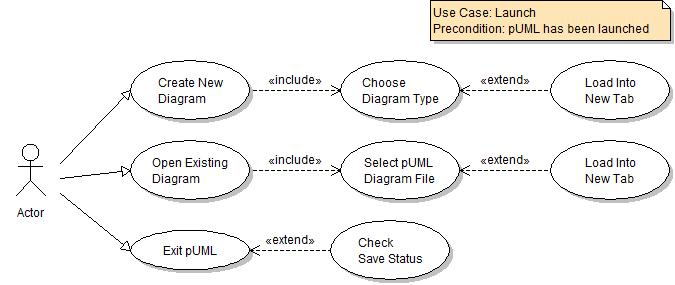
\includegraphics[width=6.0in]{ucaseLaunch.jpg}
\caption{Launch Use Case}
\end{figure}

%%% CREATE NEW PROJECT USE CASE DESCRIPTION
\begin{flushleft}
\tablehead{}
\begin{tabular}{|m{2.0in} m{5.0in}|}
\hline
{\bfseries\emph{Use Case Name}}
& {\bfseries
Create New Project}
\\\hline
\emph{Details}
& TBD
\\\hline
\end{tabular}
\end{flushleft}
\bigskip

%%% OPEN PROJECT USE CASE DESCRIPTION
\begin{flushleft}
\tablehead{}
\begin{tabular}{|m{2.0in} m{5.0in}|}
\hline
{\bfseries\emph{Use Case Name}}
& {\bfseries Open Project}
\\\hline
\emph{Details}
& TBD
\\\hline
\end{tabular}
\end{flushleft}
\bigskip

%%% EXIT PROGRAM USE CASE DESCRIPTION
\begin{flushleft}
\tablehead{}
\begin{tabular}{|m{2.0in} m{5.0in}|}
\hline
{\bfseries\emph{Use Case Name}}
& {\bfseries Exit Program}
\\\hline
\emph{Participating Actor}
& User
\\\hline
\multirow{2}{*}{\emph{Flow of Events}}
& 1. User clicks X \\
& 2. If file is not saved, include Save File As use case \\
& 3. Program Exits \\\hline
\emph{Entry Condition}
&
User initiates File menu option Close Program or clicks X in the corner of the window.
\\\hline
\emph{Exit Condition}
& File is successfully saved and the program exits.
\\\hline
\emph{Quality Requirements}
& TBD
\\\hline
\end{tabular}
\end{flushleft}
\bigskip

\clearpage

% ************************************
% NEW PROJECT USE CASE & DESCRIPTIONS
% ************************************
\paragraph[\ Use Category]
{\ New Project} 
{The user has selected to start a new UML project.}

\begin{figure}[h]
\centering
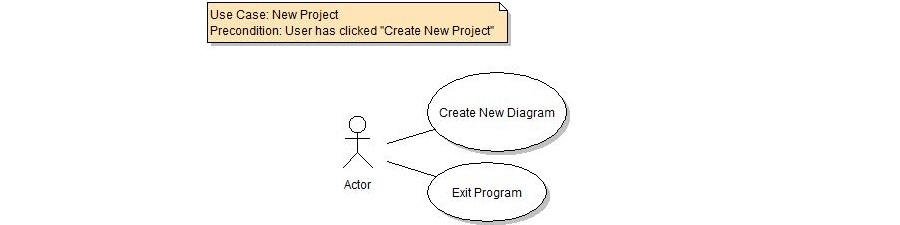
\includegraphics[width=6.0in]{ucaseNewProj.jpg}
\caption{New Project Use Case}
\end{figure}

%%% CREATE NEW DIAGRAM USE CASE DESCRIPTION
\begin{flushleft}
\tablehead{}
\begin{tabular}{|m{2.0in} m{5.0in}|}
\hline
{\bfseries\emph{Use Case Name}}
& {\bfseries New Diagram }
\\\hline
\emph{Participating Actor}
& User
\\\hline
\multirow{2}{*}{\emph{Flow of Events}}
& 1.  The user selects new file from menu \\
& 2.  Program requests user select a diagram type
(includes ChooseDiagramType use case) \\
& 3.  The program responds by creating a new file with a blank drawing canvas
\\\hline
\emph{Entry Condition}
& User selects New File from commands
\\\hline
\emph{Exit Condition}
& Program successfully opens new file
\\\hline
\emph{Quality Requirements}
& TBD
\\\hline
\end{tabular}
\end{flushleft}
\bigskip

%%% CHOOSE DIAGRAM TYPE USE CASE DESCRIPTION
\begin{flushleft}
\tablehead{}
\begin{tabular}{|m{2.0in} m{5.0in}|}
\hline
{\bfseries\emph{Use Case Name}}
& {\bfseries Choose Diagram Type}
\\\hline
\emph{Participating Actor}
& User 
\\\hline
\multirow{2}{*}{\emph{Flow of Events}}
& 1.  User selects a diagram type \\
& 2.  Program loads and displays only objects for the selected diagram type
\\\hline
\emph{Entry Condition}
& Included from New Diagram use case
\\\hline
\emph{Exit Condition}
& Included from New Diagram use case
\\\hline
\emph{Quality Requirements}
& TBD
\\\hline
\end{tabular}
\end{flushleft}
\bigskip

\clearpage


% ************************************
% OPEN PROJECT USE CASE & DESCRIPTIONS
% ************************************
\paragraph[\ Use Category]
{\ Open Project} {These options will be available to the user after choosing to open an existing UML project.}

\begin{figure}[h]
\centering
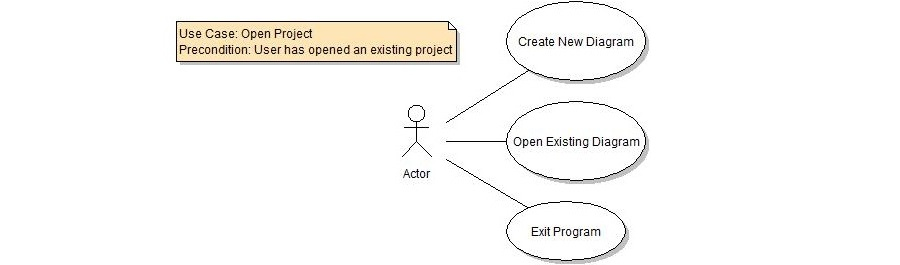
\includegraphics[width=6.0in]{ucaseOpenProj.jpg}
\caption{Open Project Use Case}
\end{figure}

%%% OPEN EXISTING DIAGRAM USE CASE DESCRIPTION
\begin{flushleft}
\tablehead{}
\begin{tabular}{|m{2.0in} m{5.0in}|}
\hline
{\bfseries\emph{Use Case Name}}
& {\bfseries Open Diagram}
\\\hline
\emph{Participating Actor}
& User
\\\hline
\multirow{2}{*}{\emph{Flow of Events}}
& 1. User selects Open File from menu \\
& 2. Program opens an explorer window \\
& 3. User selects a file \\
& 4. Program loads selected file into program \\\hline
\emph{Entry Condition}
& User selects Open File from menu.
\\\hline
\emph{Exit Condition}
& File is successfully opened.
\\\hline
\emph{Quality Requirements}
& User selected file must be able to be opened in pUML.
\\\hline
\end{tabular}
\end{flushleft}
\bigskip

\clearpage

% ************************************
% NEW DIAGRAM USE CASE & DESCRIPTIONS
% ************************************
\paragraph[\ Use Category]
{\ New Diagram} {These options will be available to the user upon choosing to create a new UML diagram.}

\begin{figure}[h]
\centering
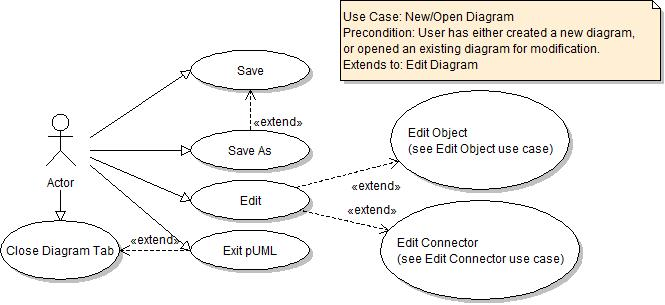
\includegraphics[width=6.0in]{ucaseNewOpenDiagram.jpg}
\caption{New/Open Diagram Use Case}
\end{figure}

%%% SAVE DIAGRAM USE CASE DESCRIPTION
\begin{flushleft}
\tablehead{}
\begin{tabular}{|m{2.0in} m{5.0in}|}
\hline
{\bfseries\emph{Use Case Name}}
& {\bfseries Save File}
\\\hline
\emph{Participating Actor}
& User
\\\hline
\multirow{2}{*}{\emph{Flow of Events}}
& 1. The user selects save file \\
& 2. Program saves file \\
& a. If file has not been previously saved, ask user where to save \\
& b. If file has been previously saved, ask user where to save
\\\hline
\emph{Entry Condition}
& User selects Save File from main menu or clicks save button.
\\\hline
\emph{Exit Condition}
& File is successfully saved
\\\hline
\emph{Quality Requirements}
& TBD
\\\hline
\end{tabular}
\end{flushleft}
\bigskip


%%% SAVE DIAGRAM AS USE CASE DESCRIPTION
\begin{flushleft}
\tablehead{}
\begin{tabular}{|m{2.0in} m{5.0in}|}
\hline
{\bfseries\emph{Use Case Name}}
& {\bfseries Save As}
\\\hline
\emph{Details}
& TBD
\\\hline
\end{tabular}
\end{flushleft}
\bigskip


%%% PRINT DIAGRAM USE CASE DESCRIPTION
\begin{flushleft}
\tablehead{}
\begin{tabular}{|m{2.0in} m{5.0in}|}
\hline
{\bfseries\emph{Use Case Name}}
& {\bfseries Print Diagram}
\\\hline
\emph{Participating Actor}
& User
\\\hline
\multirow{2}{*}{\emph{Flow of Events}}
& 1.  User initiates print. \\
& 2.  Program sends to printer
\\\hline
\emph{Entry Condition}
& User initiates Print
\\\hline
\emph{Exit Condition}
& Diagram successfully sent to printer
\\\hline
\emph{Quality Requirements}
& TBD
\\\hline
\end{tabular}
\end{flushleft}
\bigskip

%%% CLOSE DIAGRAM/TAB USE CASE DESCRIPTION
\begin{flushleft}
\tablehead{}
\begin{tabular}{|m{2.0in} m{5.0in}|}
\hline
{\bfseries\emph{Use Case Name}}
& {\bfseries Close Diagram}
\\\hline
\emph{Details}
& TBD
\\\hline
\end{tabular}
\end{flushleft}
\bigskip

%%% UNDO USE CASE DESCRIPTION
\begin{flushleft}
\tablehead{}
\begin{tabular}{|m{2.0in} m{5.0in}|}
\hline
{\bfseries\emph{Use Case Name}}
& {\bfseries Undo}
\\\hline
\emph{Details}
& TBD
\\\hline
\end{tabular}
\end{flushleft}
\bigskip

%%% REDO USE CASE DESCRIPTION
\begin{flushleft}
\tablehead{}
\begin{tabular}{|m{2.0in} m{5.0in}|}
\hline
{\bfseries\emph{Use Case Name}}
& {\bfseries Redo}
\\\hline
\emph{Details}
& TBD
\\\hline
\end{tabular}
\end{flushleft}
\bigskip


\clearpage

% ************************************
% EDIT OBJECT USE CASE & DESCRIPTIONS
% ************************************
\paragraph[\ Use Category]
{\ Edit Object} {These options will be available to the user with a diagram open for modification, who is choosing to take action on an object.}

\begin{figure}[h]
\centering
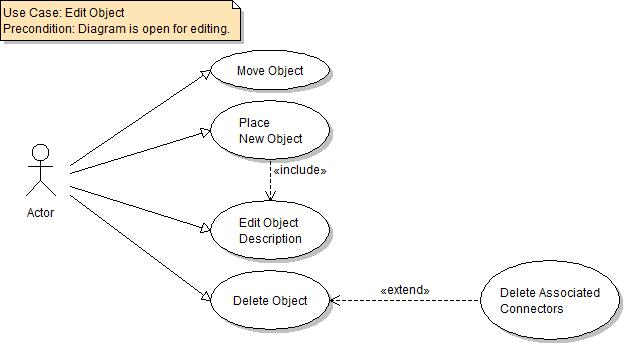
\includegraphics[width=6.0in]{ucaseEditObj.jpg}
\caption{Edit an Object Use Case}
\end{figure}

%%% PLACE NEW OBJECT USE CASE DESCRIPTION
\begin{flushleft}
\tablehead{}
\begin{tabular}{|m{2.0in} m{5.0in}|}
\hline
{\bfseries\emph{Use Case Name}}
& {\bfseries Place New Object}
\\\hline
\emph{Participating Actor}
& User
\\\hline
\multirow{2}{*}{\emph{Flow of Events}}
& 1.  User selects an object from a valid list of objects \\
& 2.  User places object on canvas.
\\\hline
\emph{Entry Condition}
& Toolbar is loaded with valid objects for diagram type
\\\hline
\emph{Exit Condition}
& Object has been successfully placed on drawing canvas.
\\\hline
\emph{Quality Requirements}
& TBD
\\\hline
\end{tabular}
\end{flushleft}
\bigskip

%%% MOVE OBJECT USE CASE DESCRIPTION
\begin{flushleft}
\tablehead{}
\begin{tabular}{|m{2.0in} m{5.0in}|}
\hline
{\bfseries\emph{Use Case Name}}
& {\bfseries Edit Object}
\\\hline
\emph{Details}
& TBD
\\\hline
\end{tabular}
\end{flushleft}
\bigskip

%%% EDIT OBJECT DESCRIPTION USE CASE DESCRIPTION
\begin{flushleft}
\tablehead{}
\begin{tabular}{|m{2.0in} m{5.0in}|}
\hline
{\bfseries\emph{Use Case Name}}
& {\bfseries Move Object}
\\\hline
\emph{Details}
& TBD
\\\hline
\end{tabular}
\end{flushleft}
\bigskip

\clearpage

% ************************************
% EDIT CONNECTOR CASE & DESCRIPTIONS
% ************************************
\paragraph[\ Use Category]
{\ Edit Connector} {These options will be available to the user with a diagram open for modification, who is choosing to take action regarding a connector.}

\begin{figure}[h]
\centering
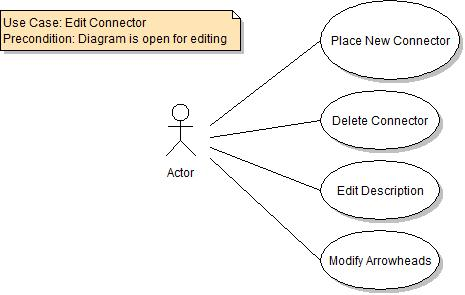
\includegraphics[width=6.0in]{ucaseEditConn.jpg}
\caption{Edit a Connector Use Case}
\end{figure}

%%% PLACE NEW CONNECTOR USE CASE DESCRIPTION
\begin{flushleft}
\tablehead{}
\begin{tabular}{|m{2.0in} m{5.0in}|}
\hline {\bfseries\emph{Use Case Name}}
& {\bfseries Place New Connector}
\\\hline
\emph{Details}
& TBD
\\\hline
\end{tabular}
\end{flushleft}
\bigskip
	

%%% EDIT CONNECTOR DESCRIPTION USE CASE DESCRIPTION
\begin{flushleft}
\tablehead{}
\begin{tabular}{|m{2.0in} m{5.0in}|}
\hline {\bfseries\emph{Use Case Name}}
& {\bfseries Edit Connector Description}
\\\hline
\emph{Details}
& TBD
\\\hline
\end{tabular}
\end{flushleft}
\bigskip

%%% DELETE CONNECTOR USE CASE DESCRIPTION
\begin{flushleft}
\tablehead{}
\begin{tabular}{|m{2.0in} m{5.0in}|}
\hline {\bfseries\emph{Use Case Name}}
& {\bfseries Delete Connector}
\\\hline
\emph{Details}
& TBD
\\\hline
\end{tabular}
\end{flushleft}
\bigskip


\clearpage






\clearpage


\subsubsection[System feature: [Project management tasks suite]{\rmfamily\bfseries System
feature: Project management tasks suite}

\paragraph[\ Introduction/Purpose of this feature]{\foreignlanguage{english}{\ }\foreignlanguage{english}{Introduction/Purpose of this feature}}
{
Several processes are required to manage projects. These include the saving of files, loading projects from files, and deleting projects.}


\paragraph[Input/Output sequence for this feature]{\rmfamily\bfseries
Input/Output sequence for this feature}
{
The user selects the "File" pull down menu at the top left corner of his or her screen. The options currently supported are "New", "Open", "Revert", "Copy As", "Save", "Save As", and "Delete Project". }

\subparagraph{New}
{
This creates a new project space. The user shall be presented with a dialog option to save the previous project. Once completing this dialog, the previous project will be closed and a new project space will be created. }

\subparagraph{Open}
{
This opens a previously saved project. The user shall be presented with a dialog option to save the previous project. Once completing this dialog, the previous project will be closed and the selected project will be opened.}

\subparagraph{Revert}
{
This disregards all unsaved changes made to the project and reverts to the saved version. A confirmation dialog shall be presented to the user before this action is completed.}

\subparagraph{Copy As}
{
This creates a new project space. First, the program will be saved. Then the user shall be presented with a dialog to choose a unique name for the new project space. Once completing this dialog, a copy of the previous project will be cloned into the new project space. The previous project shall be closed and the new project shall be opened.}

\subparagraph{Save}
{
This saves the current state of the project into an XML that can later be used to recreate the project state. If the current project does not have a name, the "Save" option will be an alias for the "Save As" option.}

\subparagraph{Save As}
{
This creates a new project space and then saves the project state into the new project. In contrast with "Copy As", this option does not affect the previous project. }

\subparagraph{Delete Project}
{
This deletes the current project and all files within the project folder. The user shall be presented with a confirmation dialog before this action is completed. Upon completion, a blank and unnamed project will be active in the project window. }









\clearpage\setcounter{page}{1}\pagestyle{Convertvi}
\section[REQUIREMENTS TRACEABILITY]{\rmfamily\bfseries
REQUIREMENTS TRACEABILITY}
{\itshape
This section shall contain traceability information from each system
requirement in this specification to the system (or subsystem, if
applicable) requirements it addresses. \ A tabular form is preferred,
but not mandatory.}


\bigskip

\begin{flushleft}
\tablehead{\hline
\multicolumn{1}{|m{0.9212598in}|}{\centering
\bfseries Feature Name} &
\centering \bfseries Req No. &
\centering \bfseries Requirement
Description &
\centering \bfseries Priority &
\centering \bfseries SDD &
\multicolumn{2}{m{1.2872598in}|}{\centering
\bfseries Alpha Release} &
\multicolumn{2}{m{1.3587599in}|}{\centering
\bfseries Beta Release} &
\multicolumn{2}{m{1.3795599in}|}{\centering
\bfseries Final Test}\\\hline
 &
 &
 &
 &
 &
\centering \bfseries Test Case(s) &
\centering \bfseries Test Res. &
\centering \bfseries Test Case(s) &
\centering \bfseries Test Res. &
\centering \bfseries Test Case(s) &
\bfseries Test
Res.\\\hhline{~~~~~------}}
\begin{supertabular}{m{0.9212598in}|m{0.42125985in}|m{1.9212599in}|m{0.39275986in}|m{0.7587598in}|m{0.6622598in}|m{0.5462598in}|m{0.6712598in}|m{0.6087598in}|m{0.6712598in}|m{0.6295598in}|}
\multicolumn{1}{|m{0.9212598in}|}{~Select Diagram Type
} &
\centering  1.1 &
~Selects the appropriate diagram type
 &
~M
 &
~N/A
 &
~N/A
 &
~N/A
 &
~N/A
 &
~N/A
 &
~N/A
 &

~N/A
\\\hline
\multicolumn{1}{|m{0.9212598in}|}{~Save function
} &
\centering  2.1 &
~Saves the Diagram to file
 &
~M
 &
~N/A
 &
~N/A
 &
~N/A
 &
~N/A
 &
~N/A
 &
~N/A
 &
~N/A
 
\\\hline
\multicolumn{1}{|m{0.9212598in}|}{~Draw function
} &
\centering  2.1 &
~Draws current objects
 &
~M
 &
~N/A
 &
~N/A
 &
~N/A
 &
~N/A
 &
~N/A
 &
~N/A
 &
~N/A

\\\hline
\multicolumn{1}{|m{0.9212598in}|}{~Open File
} &
\centering  2.1 &
~Opens previously saved file
 &
~M
 &
~N/A
 &
~N/A
 &
~N/A
 &
~N/A
 &
~N/A
 &
~N/A
 &
~N/A

\\\hline
\multicolumn{1}{|m{0.9212598in}|}{~New File
} &
\centering  2.1 &
~Creates New File
 &
~M
 &
~N/A
 &
~N/A
 &
~N/A
 &
~N/A
 &
~N/A
 &
~N/A
 &
~N/A

\\\hline

\multicolumn{1}{|m{0.9212598in}|}{~SSRS and SSDD
} &
\centering  2.1 &
~Too much work.
 &
~M
 &
~N/A
 &
~N/A
 &
~N/A
 &
~N/A
 &
~N/A
 &
~N/A
\\\hline

\end{supertabular}
\end{flushleft}
{
Priorities are: \textbf{M}andatory, \textbf{L}ow, \textbf{H}igh}

{
SDD link is version and page number or function name.}

{
Test cases and results are file names and \textbf{P}ass/\textbf{F}ail or
\% passing.}


\end{document}